\documentclass[11pt,a4paper]{article}
\usepackage[utf8]{inputenc}
\usepackage[spanish]{babel}
\usepackage{amsmath}
\usepackage{amsfonts}
\usepackage{amssymb}

\usepackage{hyperref}
\usepackage{graphicx}
\usepackage{geometry}
\usepackage{apacite}

\usepackage{listings}
\usepackage{xcolor}

\newgeometry{left=3cm, right=3cm, top=2.5cm, bottom=2.5cm}

\definecolor{codegreen}{rgb}{0,0.6,0}
\definecolor{codegray}{rgb}{0.5,0.5,0.5}
\definecolor{codepurple}{rgb}{0.58,0,0.82}
\definecolor{backcolour}{rgb}{0.95,0.95,0.92}

\lstdefinestyle{mystyle}{
	backgroundcolor=\color{backcolour},   
	commentstyle=\color{codegreen},
	keywordstyle=\color{magenta},
	numberstyle=\tiny\color{codegray},
	stringstyle=\color{codepurple},
	basicstyle=\ttfamily\footnotesize,
	breakatwhitespace=false,         
	breaklines=true,                 
	captionpos=b,                    
	keepspaces=true,                 
	numbers=left,                    
	numbersep=5pt,                  
	showspaces=false,                
	showstringspaces=false,
	showtabs=false,                  
	tabsize=2
}

\begin{document}
\begin{titlepage}
\centering


{\bfseries\LARGE UNIVERSIDAD NACIONAL DEL ALTIPLANO\par}
{\scshape\LARGE Facultad de Ingeniería Mecánica Eléctrica, Electrónica y Sistemas\par}
{\scshape\LARGE Escuela Profesional de Ingeniería de Sistemas\par}
\vspace{1cm}
{
\includegraphics[width=0.5\textwidth]{images/1-unap.png}\par}
\vspace{0.5cm}
{\bfseries\LARGE EVALUACIÓN DE PROGRAMACIÓN ORIENTADA A OBJETOS EN C++\par}
\vspace{1cm}
{\LARGE Docente: Mg. Aldo Hernan Zanabria Galvez \par}
{\LARGE Alumno: Yoel Nhelio Canaza Chagua \par}
\vspace{1cm}
{\LARGE Curso: \par}
{\LARGE Programación Orientada a Objetos II \par}
\vspace{1cm}
{\LARGE CICLO III – SEMESTRE 2023 – II \par}
{\LARGE PUNO, PERÚ \par}
{\LARGE 2023 \par}


\end{titlepage}

\section{Pregunta 1: Conceptos Básicos}
\subsection{Herencia: ¿Qué es la herencia en C++ y cuál es su propósito principal en la programación orientada a objetos?}

La herencia es un concepto que permite la creación de nuevas clases tomando como base clases ya existentes. Una clase puede heredar los atributos y métodos de otra clase, llamada clase base, y luego extender o modificar esa funcionalidad para adaptarla a sus propias necesidades.

Se puede comparar la herencia con la relación entre padres e hijos. Un hijo hereda ciertos rasgos y características de sus padres, pero también puede desarrollar sus propias características únicas.
\\ \\
El propósito principal de la herencia en la programación orientada a objetos es:

\begin{itemize}
\item Reutilizar código
\item Permitir la implementación del polimorfismo
\item Permitir extender y especializar el comportamiento de la clase base según las necesidades específicas de la clase derivada.
\item Modelar relaciones jerárquicas entre conceptos del mundo real. 
\end{itemize}


\subsection{Polimorfismo: Describa qué es el polimorfismo y proporcione un ejemplo práctico en C++.}
Para explicarlo de manera sencilla imaginemos que tenemos tres elementos: una puerta, una ventana y una caja. Estos tres objetos tendrían el método abrir. En la programación orientada a objetos, cada clase de estos objetos debería saber cómo realizar esa operación.

Esta característica le permite a los objetos de diferente clase intercambiar mensajes con una misma estructura.

Algunos autores también definen el polimorfismo como "la capacidad de un objeto de tomar muchas formas".

Link al repositorio en GitHub en el que se encuentra el siguiente ejemplo: \url{https://github.com/YoelCanaza/evaluacion-poo2-1/blob/40ac42fb3afd7be90304a34d771ef4edde731d76/p-1-b.cpp}

\begin{lstlisting}[language=C++, style=mystyle, caption={Polimorfismo en C++.}]
#include <iostream>
#include <string>

using namespace std;

class Animal {
protected:
    static int numero_animales;
    string alimento;
public:
    Animal();
    ~Animal();
    static int obtenerNumeroAnimales();
   
    void comer(Animal *a){
        cout<<"Este animal esta comiendo " << a->alimento<<endl;
    };
};

int Animal::numero_animales = 0;

Animal::Animal()
{
    cout<<"Creando nuevo animal ... "<<endl;
    numero_animales += 1;
}

Animal::~Animal()
{
    cout<<"Borrando animal..."<<endl;
    numero_animales-=1;
}

int Animal::obtenerNumeroAnimales()
{
    return numero_animales;
}

class Herviboro : public Animal {
public:
    Herviboro():Animal(){
        this->alimento = "plantas ";
    }
};

class Carnivoro : public Animal {
public:
    Carnivoro():Animal(){
        this->alimento = "carne ";
    }
};

int main(){
    Animal *a = new Animal();
    Herviboro *h = new Herviboro();
    Carnivoro *c = new Carnivoro();

    cout<<"Numero de animeles: "<<Animal::obtenerNumeroAnimales()<<endl;
    
    a->comer(h); 

    a->comer(c);

    delete a;
    delete h;
    delete c;
    cout<<"Numero de animales: "<<Animal::obtenerNumeroAnimales()<<endl;
}
\end{lstlisting}

En el ejemplo anterior podemos ver que la misma función o método comer puede recibir cualquier tipo de animal, y sin importar cuál sea el tipo que reciba, va a poder obtener su nombre.



\section{Pregunta 2: Implementación de Clases \\ Implemente una clase llamada Rectangulo en C++ que represente un rectángulo. Incluya atributos para el ancho y el alto, así como métodos para calcular el área y el perímetro. Muestre un ejemplo de cómo usar esta clase en un programa principal.
}

El siguiente código se encuentra almacenado en el siguiente repositorio de GitHub: \url{https://github.com/YoelCanaza/evaluacion-poo2-1/blob/f5b87ebd5733f5e520cbce8d34dc4260370073ff/p2.cpp}

\begin{lstlisting}[language=C++, style=mystyle, caption={Implementación de clases en C++}]
#include <iostream>
using namespace std;

class Rectangulo
{
public:
    Rectangulo(float ancho, float alto);

    float area();
    float perimetro();
protected:
    float anchoR;
    float altoR;
};

Rectangulo::Rectangulo(float ancho, float alto)
    : anchoR(ancho), altoR(alto)
{
    //El cuerpo estara vacio ya que ya se inicializaron los datos miembro
}

float Rectangulo::area()
{
    return anchoR * altoR;
}

float Rectangulo::perimetro()
{
    return 2 * (anchoR + altoR);
}


int main()
{
    float ancho, alto;
    cout << "Ingrese el ancho del rectangulo: "; cin >> ancho;
    cout << "Ingrese la altura del rectangulo: "; cin>> alto;

    Rectangulo r1(ancho, alto);

    cout << "El area del rectangulo es: " << r1.area() << endl;
    cout << "El perimetro del rectangulo es: " << r1.perimetro() << endl;
}
\end{lstlisting}


\section{Pregunta 3: Uso de Punteros y Memoria Dinámica: \\ Escriba un programa en C++ que utilice punteros y memoria dinámica para crear un arreglo dinámico de enteros. Luego, realice una operación específica (por ejemplo, duplicar todos los elementos) y muestre el resultado}

El código se encuentra almacenado en: \url{https://github.com/YoelCanaza/evaluacion-poo2-1/blob/cebac1d8a3867831acfae8376a70a25059b0549f/p3.cpp}

\begin{lstlisting}[language=C++, style=mystyle, caption={Pregunta 3}]
#include <iostream>

using namespace std;

int main() {
    int tamano;

    cout << "Ingrese el tamanio que tendra el arreglo: ";
    cin >> tamano;

    int* arreglo = new int[tamano];

    cout << "Ingrese los elementos del arreglo:" << endl;
    for (int i = 0; i < tamano; i++) {
        cout << "Elemento " << i + 1 << ": "; cin >> arreglo[i];
    }

    for (int i = 0; i < tamano; ++i) {
        arreglo[i] *= 2;
    }

    cout << "Arreglo con todos sus elementos duplicadoss:" << endl;
    for (int i = 0; i < tamano; i++) {
        cout << arreglo[i] << " ";
    }
    cout << endl;

    delete[] arreglo;

}
\end{lstlisting}

{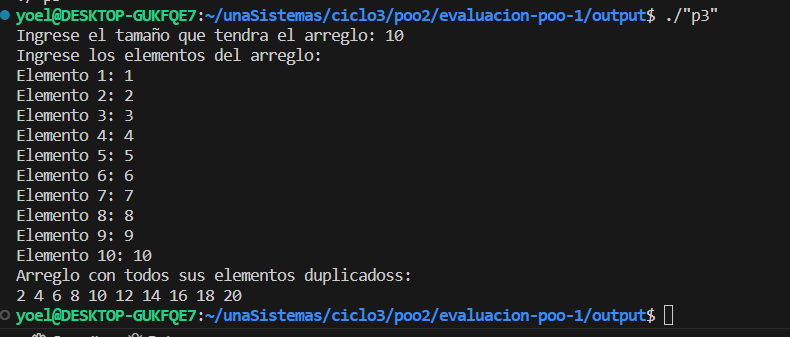
\includegraphics[width=1\textwidth]{images/2-compilado.png}\par}



\section{Pregunta 4: Manejo de Excepciones}
El manejo de excepciones en C++ es una técnica que permite lidiar con situaciones excepcionales o errores durante la ejecución de un programa. Una excepción es básicamente una señal de que algo inesperado ha ocurrido, y el manejo de excepciones proporciona una forma estructurada de gestionar estas situaciones.


\end{document}